\subsubsection{Salīdzinājums} \label{sec:fast-compare}
Iepriekš apskatīto implementāciju salīdzināšana nav triviāls uzdevums.
Pat salīdzinot tikai CPU implementācijas, tika iegūti nekonsistenti
rezultāti (sk.~\ref{fig:test1-data-txt}~att.).
\begin{figure}[tbh]
	\centering
	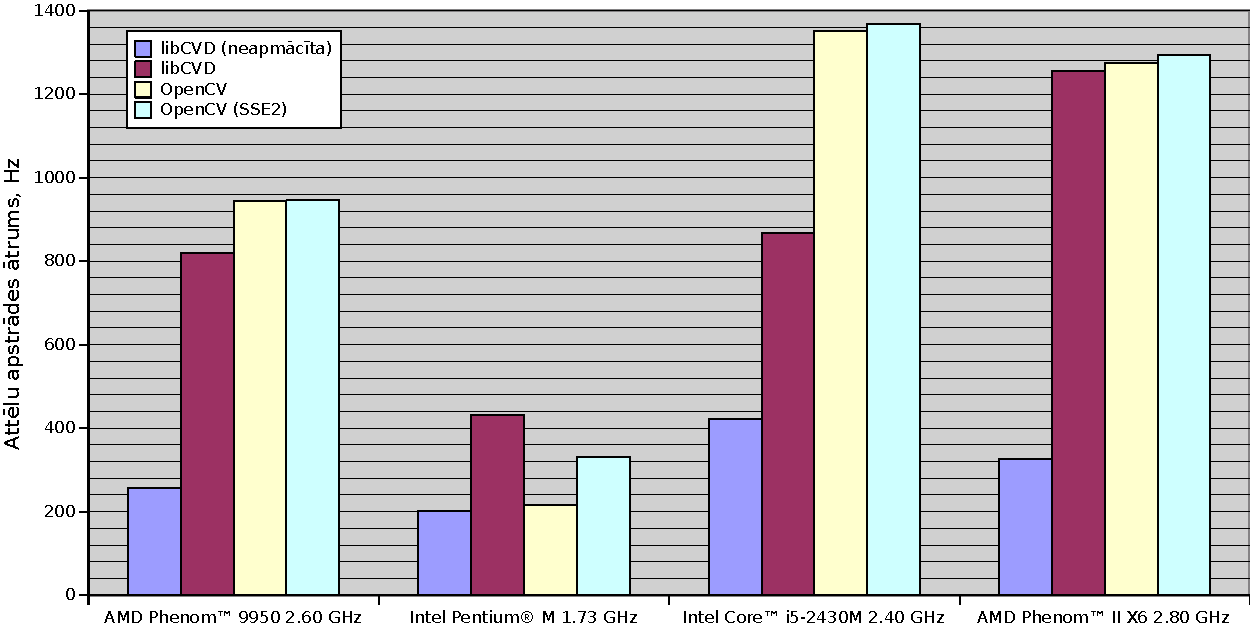
\includegraphics[width=\linewidth]{chart-cpu}
	\caption{CPU implementāciju ātrdarbības salīdzinājums.}
	\label{fig:test1-data-txt}
\end{figure}
Vecākas paaudzes Pentium procesoram labākais ātrdarbības rādītājs bija tieši
mašīnmācāmajai (libCVD) FAST implementācijai, savukārt jaunāko paaudžu
procesoriem labāku ātrdarbību uzrādīja OpenCV SSE2 uzlabotā implementācija.
AMD~Phenom~II gadījumā libCVD un OpenCV SSE2 implementācijas uzrādīja
līdzvērtīgu rezultātu.
Šādi rezultāti skaidrojami, galvenokārt, ar SSE2 veiktspējas uzlabojumiem
jauno paaudžu procesoriem~\cite{Core2}. Papildus tam, mašīnmācāmā FAST
implementācijas jautājumu koks veido apjomīgu mašīnkodu ar lielu skaitu
zarošanos. Koda apjoms un nelineārā izpildes secība samazina izpildes koda
lokalitāti un ierobežo instrukciju kešatmiņas efektivitāti.

